\chapter{Better Resizable Arrays}

\section{Hashed Array Tree (Sitarski, 1996)}

\begin{tcolorbox}[title=Terminology]
	To avoid confusion, we will use the following definitions for \textit{size} and \textit{capacity}:
	\begin{itemize}
		\item \textbf{Size} refers to the number of elements in a data structure (often denoted as $n$ or $N$)
		\item \textbf{Capacity} refers to the maximum number of elements a data structre can hold
	\end{itemize}
\end{tcolorbox}

\subsection*{Structure}

\begingroup

\begin{wrapfigure}{l}{0.4\textwidth}
	\centering
	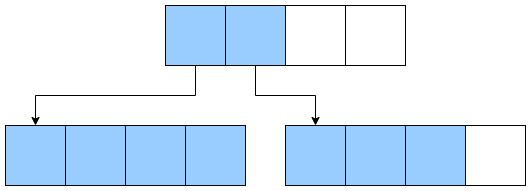
\includegraphics[width=0.4\textwidth]{01/structure.png}
    \caption{HAT with $B=4$}\label{hashed-tree-diagram}
\end{wrapfigure}
Despite the name, hashed array trees (HAT) have nothing to do with hashing or trees. Instead, it is more
akin to a 2D array$-$a 2-level structure where the first level (\textit{Top}) keeps track of the 
second level (\textit{Leaf/Leaves}). The the capacity of the Top array and each Leaf are dictated
by $B$, an integer $\geq1$. For the sake of simplicity, we will also assume that $B$ is always
a power of two.

Since both Top and Leaf each has a capacity of $B$, the entire HAT has a capacity of $B^2$.
Let $n$ be the size of the entire HAT.
\begin{equation}\label{hat-invariant}
	\left(\frac{B}{4}\right)^2 \leq n \leq B^2
\end{equation}
The proof for this will come later on in the notes when we look at expanding and shrinking HATs.

\endgroup

\subsection*{Resizing}

\begingroup

When a HAT is full, its policy for growing is by doubling $B$ and copying data over. This achieves
a couple things. It ensures that $B$ is still a power of 2. It also quadruples the capacity of the
HAT. Suppose that the current capacity of the HAT is $N$, the new capacity will be
\[(2B)^2 = 4B^2 = 4N \]

Conversely, $B$ is halved when a HAT becomes too sparse. Here, we define a sparse HAT to be a HAT 
where the number of elements $N \leq (B/4)^2$. Suppose that the current capacity of the HAT is $N$,
the new capacity will become 

\endgroup

\subsection*{Accessing an Element}

\begingroup

Suppose we are trying to access element $e$ at index $i$. We need to compute an index for Top to get
the right Leaf, then compute another index for the Leaf to get $e$. The index for Top and Leaf can
be computed by $\floor{i/B}$ and $i \pmod B$ respectively.

Since division and modulo are rather expensive operations, there are ways to speed these operations
up. Recall the assumption that $B$ is always a power of 2, meaning $B = 2^k$ for some
positive integer $k$. $\floor{i/B}$ can now be simply computed by \mintinline{c}{i >> k}. 
Additionally, the same property also simplifies the modulo operation as it can be computing by
\mintinline{c}{i & (1 << k - 1)}.

\endgroup

\subsection*{Space Analysis}

\begingroup

\begin{wrapfigure}{r}{0.4\textwidth}
	\vspace*{-10pt}
	\centering
	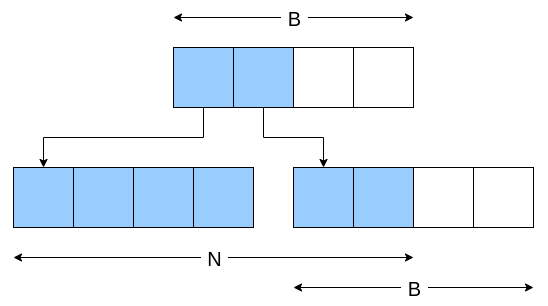
\includegraphics[width=0.4\textwidth]{01/space.png}
	\caption{Space usage of a HAT}
	\vspace*{-30pt}
\end{wrapfigure}

Consider a HAT with size $N$ and an arbitrary $B$. We need $B$ \textit{slots} to be the Top array,
$N$ slots for the elements themselves, and at most another $B$ slots for the Leaf that is not full
yet. Therefore, the space usage of the HAT is $N + 2B$. Recall that $N = B^2$, we can also rewrite
the space usage as $N + 2\sqrt{N} = N + O(\sqrt{N})$.

\subsection*{Amortized Time Analysis}

Consider a full HAT of size $N$ and some arbitrary $B$. For the sake of simplicity, let us assume
that the memory allocation is magically instantaneous. This means that, on average, each append
operation would be constant time since writing to an array takes constant time as well.
Thus, the growing cost comes mainly from copying the $N$ elements over from the old HAT
to the new one.

Since we only expand the HAT ever so often, we would have \textit{cheap} operations to make up for 
the expensive expansion operations. In order to find the number of cheap append operations between
expansions, we can simply compute the difference between the capacity of each expansion. Since $B$
is doubled in each expansion, we know that the $B$ before the last expasion would be half of the
current one. Therefore, we can compute the following to get the difference.
\[ B^2 - \left(\frac{B}{2}\right)^2 \]
This can then be rewritten in terms of $N$ and we will obtain.
\[ N - \frac{N}{4} = \frac{3}{4}N \]

Therefore, the amortized cost per append operation would be constant time.
\[ \frac{N}{(3/4)N} = \frac{4}{3} \in O(1) \]

\endgroup

\begin{tcolorbox}[title=Disclaimer]
	The naming for the following sections are not based on the original papers. These are named
	such that they are distinguishable from one another and makes sense and \textit{saves me 
	from having to write optimal resizable arrays every time I mention it}.
\end{tcolorbox}

\begingroup

\section{Fancier HAT (Brodnik et al., 1996)}

While Sitarski's HAT idea is able to achieve a better space bound than a typical resizable array,
any resize operation still takes $O(N)$ where $N$ is the capacity of the HAT before the resize.
Brodnik et al.'s idea, however, proposes a data structure that is able to achieve a constant
running time on expansion and shrinking operations.

\subsection*{Structure}

\begin{wrapfigure}[10]{L}{0.35\textwidth}
	\centering
	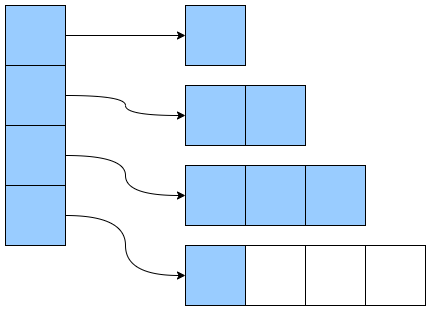
\includegraphics[width=0.35\textwidth]{01/basic-fancy-hat.png}
	\caption{Fancy HAT with $B=4$}\label{basic-fancy-hat}
\end{wrapfigure}

Brodnik et al. first proposes a similar idea to Sitarski's HAT where the data structure keeps an 
index block and many data blocks. The capacity of the data blocks ranges from 1 to $B$, and there 
are $B$ data blocks being pointed to from the index block. Here, the $i$-th block has a capacity of
$i$. This mean that the capacity of the entire data structure is $B(B+1)/2$. This is approximately
$\Theta(\sqrt{N})$ where $N$ is the capacity of the entire data structure.

\subsection*{Accessing an Element}

The problem with this data structure is the index for the index block is computed by 
\[ \ceil{\frac{\sqrt{8i + 1} - 1}{2}} \]
which has to compute the square root. Even with Newton's method, the running time is still not
constant, therefore making any access take non-constant time which doesn't improve on Sitarski's idea.

\endgroup

\begingroup

\section{Super HAT (Brodnik et al., 1999)}

\begin{wrapfigure}[16]{l}{0.4\textwidth}
	\centering
	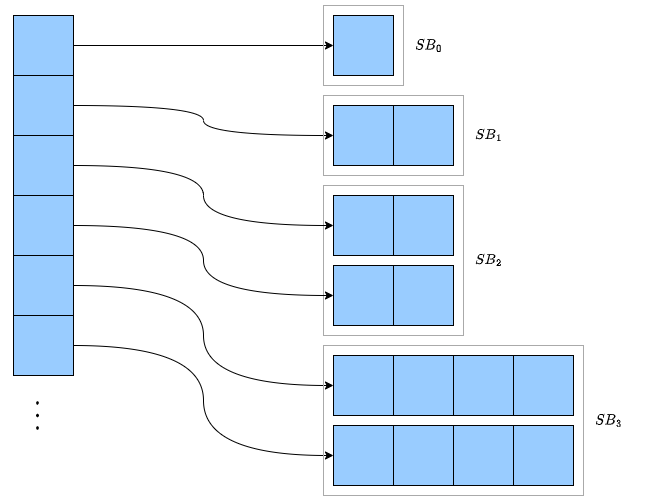
\includegraphics[width=0.4\textwidth]{01/super-hat.png}
	\caption{Super HAT}\label{super-hat-structure}
\end{wrapfigure}

\subsection*{Structure}

The basic structure is similar to the Fancy HAT but the capacity of any data block is a power of 2.
These data blocks are also clustered into \textbf{super blocks} with the following policies: two
data blocks are in the same super block if they have the same size the $k$-th, each super block
contains up to $2^\floor{k/2}$ data blocks, and each data block in each super block has a 
capacity of $2^\ceil{k/2}$.

\subsection*{Accessing an Element}

Using the properties that come from super blocks, using bit operations for computing the index for
the index block is now \textit{somehow} possible. Note that the index for the super block starts
from 0, not 1.

\endgroup
